\section{Datawarehouse}

Here's a possible star-schema for the data warehouse:


\begin{figure}[H]
    \centering
    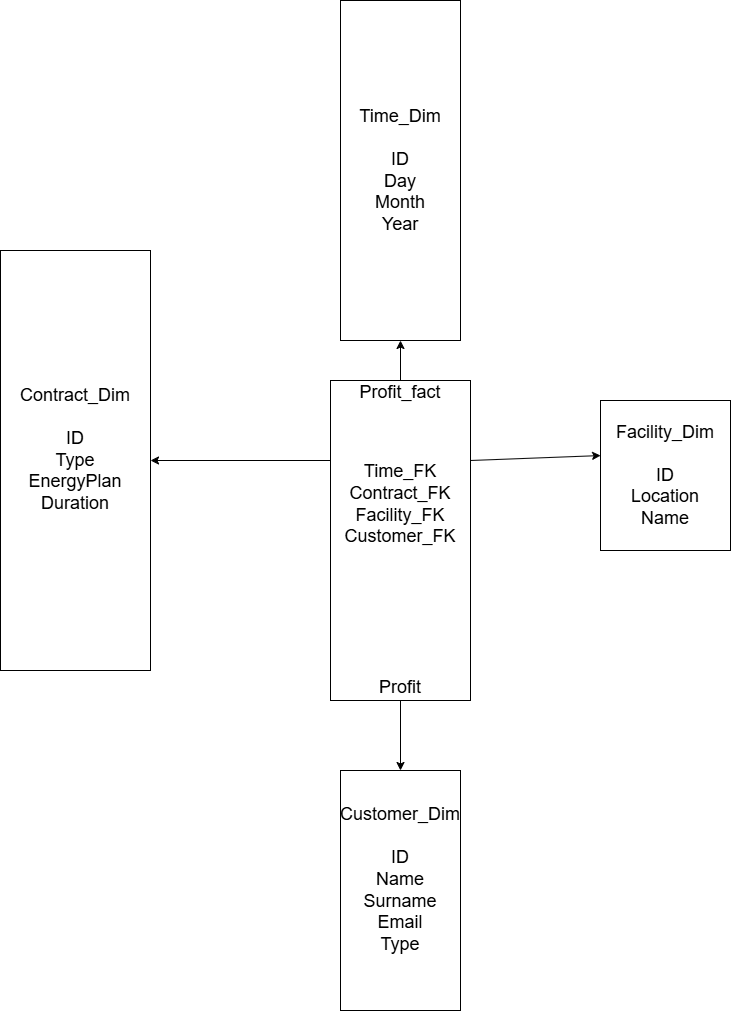
\includegraphics[width=\textwidth,height=0.7\textheight]{images/Fact1.png}
    \caption{Fact: Profit}
\end{figure}

\noindent In this example the main fact is the profit. We can analize it in different ways. Examples:
\begin{itemize}
    \item Profit by type of contract: what type of contract is more profitable?
    \item Profit by customer: who are the most profitable customers?
    \item Profit by Facility: which facilities are more profitable?
    \item Combined analysis: what type of contract is more profitable for a specific facility?
\end{itemize}

\begin{figure}[H]
    \centering
    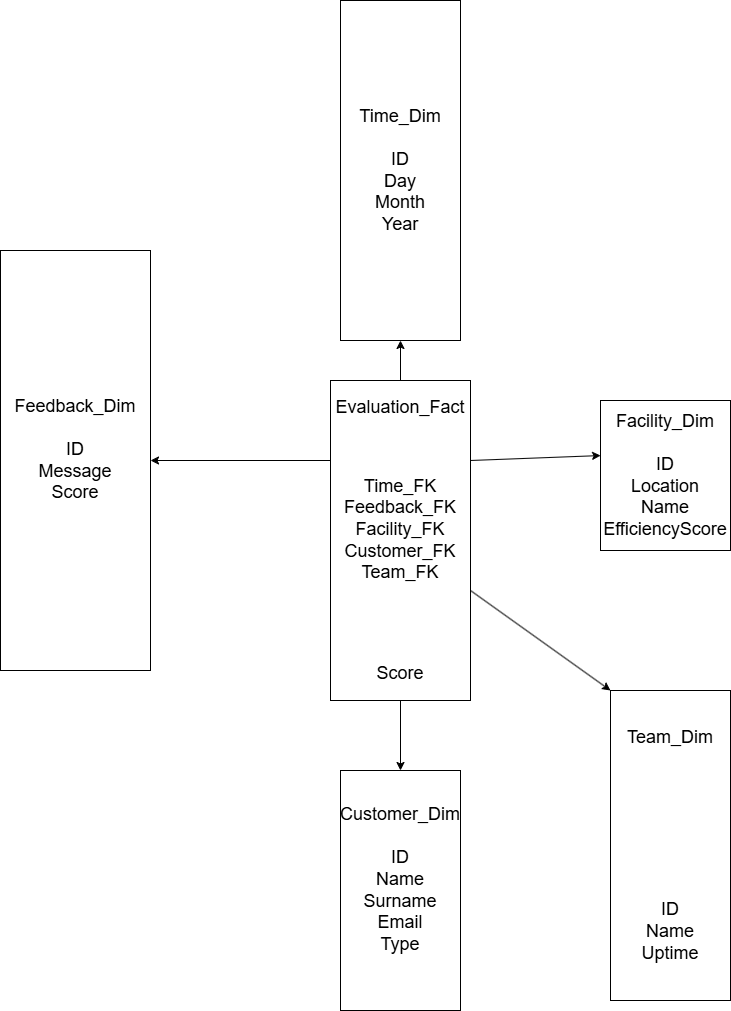
\includegraphics[width=\textwidth,height=0.7\textheight]{images/Fact2.png}
    \caption{Fact: Evalutation}
\end{figure}

\noindent In this example the main fact is the evaluation. We can analize it in different ways. Examples:
\begin{itemize}
    \item Which team has the best score? And the worst?
    \item On average, which component has the higher weight in the evaluation: energy efficiency, uptime, customer satisfaction?
    \item Combined analysis: what is the average evaluation of a customer?
    \item Combined analysis: has a customer have a bias in the evaluation of a specific team?
\end{itemize}
